\section{Methods}

We propose an optimization procedure that incrementally minimizes mesh vertex noises using differentiable rendering. 
Suppose we have vertices $V=\{V_i\in\mathbb{R}^3\}=\{V_0...V_n\}$ within input mesh $\mathcal{M}$ which is fused from input color $\mathcal{C}$ and depth $\mathcal{D}$ with intrinsic $K$ such that $\mathcal{M}=K^{-1}\left(\mathcal{C}\oplus \mathcal{D}\right)$. 
Here, $\oplus$ denotes image registration operator.
We define deformed vertices $V_d$, which has same shape as $V$ initialized with zero values i.e., $V_d=\{\mathbf{0}_0,...,\mathbf{0}_n\}$. 
For every iteration, $V_d$ is optimized so that resulting vertices $V_o=V+V_d$ approximate noise-free geometry which looks perceptually similar with $\mathcal{C}$. 
The main problem is how to find common geometric representations between $\mathcal{C}$ and $C$ to figure out which region is to be optimized (i.e., noisy). 

\subsection{Exploting assumptions underlying existing SLAM datasets}
We found two common aspects within $\mathcal{C}$ taken from most of SLAM dataset, which acts important role to consider $\mathcal{C}$ as geometric clue.

\noindent \textbf{Lambertian-dominant}. 
This naturally satiesfies since this is an assumption for vast majority of SLAM dataset, unless it is used for vaildating SLAM algorithm under non-Lambertian environment e.g., \cite{whelan2018reconstructing}. 
In order to track accurate camera pose during SLAM, finding reliable feature correspondences are necessary.
Generally, a point shown in two images that shares overlapped region $\mathcal{C}_0$, $\mathcal{C}_1$ is chosen, which satisfies photometric consistency e.g., $E_{photo}=\arg\min_x \mathcal{C}_0\left(x+\overrightarrow{\mathrm{u}}\right)-\mathcal{C}_1\left(x\right)$. \cite{szeliski2010computer}
This is because it has been empirically considered as 'static anchor' on a given scene; a point on a surface never deforms during capturing stage, and its value is direction-invariant so that the point has consistent pixel value wherever an image is taken from. 

Interpreting photometric consistency in computer graphics field is trivial; this indicates that a point is lie on a Lambertian surface, such that a bi-directional reflectance $f(x, w_i, w_o)=c$, where $c\le 1$ is a constant.


\noindent \textbf{No strong radiance changes within a plane}. 
We found that there seldom have strong radiance changes within a plane among indoor SLAM datasets. 
Here, a plane can be a structural information of given scene (e.g., wall, floor, ceiling), or upper part of an object (e.g., desk, box).
Although there may exists a case that a plane have strong radiance changes (e.g., chessboard pattern on floor), we decided to ignore them. 
In other words, any point within a plane have similar pixel value with neighbors lie on same plane. 
Note that our proposed method works even though this assumption does not met, however we decide to made it for the sake of ease of explanation.


\subsection{Re-vising: How Geometry Affects to Color Image}
In this section, we formally describe our intuition that enables input color image treated as noise-free geometric clue.

Let us consider $\mathcal{C}$ as a result from perfect renderer which is capable of tracing full light transport without any noise or outlier, given unknown lighting conditions and noise-free geometry. 
Based on Light Transport Equation(LTE) representation with respect to path integral form \cite{veach1998robust}, we represent $\mathcal{C}$ as a set of solution of LTE for each pixel:

\begin{align}
    \mathcal{C} & = \bigcup_i^W \bigcup_j^H L_{i,j}\left(K^{-1}\cdot x\rightarrow p_0\right) \nonumber \\
    & = \bigcup_i^W \bigcup_j^H L_{i,j}\left(p_1\rightarrow p_0\right),
    \label{eqn:color_image_rendering_equation}
\end{align}
where $L_{i,j}$ is total radiance at a pixel, and $p_1=K^{-1}\cdot x$ is a hitpoint corresponds to $L_{i,j}$.

To intuitively exploit relationship between $\mathcal{C}$ and noise-free hitpoint $x_{i,j}$, we select arbitrary pixel and its total radiance in (Eqn. \ref{eqn:color_image_rendering_equation}) and expand radiance sum over path segments $\bar{\mathrm{p}}_n=\mathrm{p}_0\mathrm{p}_1...\mathrm{p}_n$ with $n+1$ vertices:
\begin{align}
    L_{i,j}\left(p_1\rightarrow p_0\right)& = \mathit{P}\left(\bar{\mathrm{p}}_1\right)+\mathit{P}\left(\bar{\mathrm{p}}_2\right)+\sum_{n=3}^\infty \mathit{P}\left(\bar{\mathrm{p}}_n\right), 
    \label{LTE_path_integral}
\end{align}

Let us consider direct lighting term in (Eqn. \ref{LTE_path_integral}) first:

\begin{align}
    \mathit{P}\left(\bar{\mathrm{p}}_2\right) & = \int_A && f\left(\mathrm{p}_2\rightarrow \mathrm{p}_1 \rightarrow \mathrm{p}_0\right)\cdot L_{e(i,j)}\left(\mathrm{p}_2\rightarrow \mathrm{p}_1\right) \cdot G\left(\mathrm{p}_1 \leftrightarrow \mathrm{p}_2\right) \nonumber \\
    & = \int_A && \Bigg[ f\left(\mathrm{p}_2\rightarrow \mathrm{p}_1 \rightarrow \mathrm{p}_0\right)\cdot L_{e(i,j)}(\mathrm{p}_2\rightarrow \mathrm{p}_1) \nonumber \\ 
    & && \cdot V(\mathrm{p}_1 \leftrightarrow \mathrm{p}_2) \cdot \frac{|\cos(\theta_1)| |\cos(\theta_2)|}{||\mathrm{p}_1-\mathrm{p}_2||^2}\Bigg]
    \label{LTE_path_integral_direct_lighting}
\end{align}

Note that we omitted path differential $dA(\mathrm{p}_2)$ for brevity.

Since we assumed Lambertian surface and emitted radiance term is free up to any geometric transformation, the term that affects to direct lighting value in (Eqn. \ref{LTE_path_integral_direct_lighting}) is \textbf{geometry term}: visilbility, incident angles, and distance between hitpoints. \PJ{TODO: parameterize hitpoint as a sum of barycentric coords of vertex positions within a face.}

We will drop any consideration of remaining terms in (Eqn. \ref{LTE_path_integral}). We do not consider emitted radiance i.e., albedo term $\mathit{P}\left(\bar{\mathrm{p}}_1\right)$ since this represents pure physical quantity of a geometry have, thus itself is consistent up to any geometric displacement (e.g., additive noise on vertices).
\PJ{Does it sound clear?}
We additionally treat indirect lighting term $\sum_{n=3}^\infty \mathit{P}(\bar{\mathrm{p}}_n)$ as it is; we will consider that indirect lighting cannot make a pixel value strongly deviated with neighbors where is originally have similar value within neighbors when only direct lighting is applied. 
This seems feasible because (1) indirect lighting term uses identical rendering equation with direct lighting term except to hitpoints (2) its throughput is far smaller than direct lighting term, under Lambertian assumption (3) it is applied globally; to make a pixel saturated against neighbors indirect lighting have to be applied to only that pixel (4) in a photorealistic rendering domain, multiple bounces among diffuse material causes significant noise, hence often ignored\cite{moon2013robust}.

Therefore, we conclude that radiance at a pixel $L_{i,j}(p_1 \rightarrow p_2)$ is mostly affected by \textbf{geometry term} in $\mathit{P}(\bar{\mathrm{p}}_2)$ i.e., 
\begin{align}
    L_{i,j}(p_1 \rightarrow p_2) \sim \mathit{P}(\bar{\mathrm{p}}_2) & \propto G(\mathrm{p}_1 \leftrightarrow \mathrm{p}_2) \nonumber \\
    & =V(\mathrm{p}_1 \leftrightarrow \mathrm{p}_2) \cdot \frac{|\cos(\theta_1)||\cos(\theta_2)|}{||\mathrm{p}_1-\mathrm{p}_2||^2}
    \label{eqn:relationship_between_radiance_and_geometry}
\end{align}

We now examine direct lighting term in rendering $C$, where noisy geometry $\mathcal{M}$ is used.

\begin{align}
    \mathit{P}\left(\bar{\mathrm{p}}'_2\right) = c\int_A L_{e(i,j)}(\mathrm{p}'_2\rightarrow \mathrm{p}'_1) \cdot V(\mathrm{p}'_1 \leftrightarrow \mathrm{p}'_2) \cdot \frac{\left|\cos(\theta_1)'\right|\left|\cos(\theta_2)'\right|}{\left|\left|\mathrm{p}'_1-\mathrm{p}'_2\right|\right|^2} \nonumber
    \label{LTE_path_integral_direct_lighting_SLAM}
\end{align}

As $\mathcal{M}$ is composed with noisy vertices $V$, \textbf{geometry term} is highly likely to have different value against those from $\mathcal{C}$. 
Thus, there may exist different radiance values between $\mathcal{C}$ and $C$ though evaluated at an identical pixel position.

This naturally concludes that a loss minimizing radiance difference equals to matching \textbf{geometry term} in $C$ similar with $\mathcal{C}$.

However, simply minimizing color difference i.e., $||\mathcal{C}-C||^2$ does not work, as the texture of $\mathcal{M} \sim \mathcal{C}$ contains real light information, furthermore we will cast a virtual light to saturate noisy vertices. 
Therefore, $C$ have far different tone compared to $\mathcal{C}$ in a global manner. 
The main challenge is to detect geometric differences between images in a local manner, regardless of any radiance tone changes.

\subsection{Detecting Geometric Information given Color Image and Its Rendering}
In this section, we describe our method to detect geometric information in both $\mathcal{C}$ and $C$, based on our intuition in (Eqn. \ref{eqn:relationship_between_radiance_and_geometry}).

We showed that changes of value made in a pixel is proportional to geometric transformation of a corresponding hitpoint.
Consider a pair of hitpoint and corresponding pixel, together with neighboring pixels and corresponding hitpoints lie on same plane.
If pixel values are evaluated in $\mathcal{C}$, they will have similar radiance values according to assumption. 
This can be expressed as:
\begin{equation}
    |L(K^{-1}\cdot x_{i,j})-L(K^{-1}\cdot x_{i+\delta_i, j+\delta_j})| < \epsilon, 
    \label{eqn:pixel_difference_near_epsilon}
\end{equation}
where $\delta_i \neq 0, \delta_j \neq 0$ is pixel coordinate displacement indicating neighbor of a pixel.

Based on our intuition, we decided to apply image gradient kernel to detect geometric displacement. 
This is natural as image gradient saturates where pixel values are discontinuous along with a pixel and its neighbors.
From our assumption and intuition, this directly indicates that saturated region equals to the position where is geometrically discontinuous.
If we apply image gradient kernel $G(\cdot)$ to $\mathcal{C}$, $G(\mathcal{C})$ have zero values where satisfies (Eqn. \ref{eqn:pixel_difference_near_epsilon}), and vice versa.

We simply detect noise-free surfaces within $\mathcal{C}$ by applying Scharr gradient kernel. 
In order to ensure robustness on strong texture changes, one may adapt gradient from $\mathcal{D}$; note that for this report we only experimented with gradients from $\mathcal{C}$. 
Specifically, Scharr kernel for each axis over an image is defined as
\begin{equation}
    \label{eqn:01}
    G_x=\begin{pmatrix}
        -3 & 0 & 3\\
        -10 & 0 & 10\\
        -3 & 0 & 3
    \end{pmatrix}, 
    G_y=\begin{pmatrix}
        -3 & -10 & -3\\
        0 & 0 & 0\\
        3 & 10 & 3
    \end{pmatrix}
    ,
\end{equation}
and our detected geometric changes over Ground Truth color image $\widetilde{G}_\mathcal{C}$ is a Scharr gradient of $I_\mathcal{C}$ i.e., the intensity image from $\mathcal{C}$. 
Since resulting gradient on some pixels have negative value of identical magnitude to positive values of neighboring pixel, we take its absolute value
\begin{equation}
    \label{eqn:02}
    \widetilde{G}_\mathcal{C}=\frac{1}{2}\left(|G_x\left(I_\mathcal{C}\right)|+|G_y\left(I_\mathcal{C}\right)|\right)
\end{equation}
In order to detect noisy vertices on $C$ regardless of shading method, we propose Lightweight map to determine which vertex has stronger noise compare to $\widetilde{G}_\mathcal{C}$. 
Lightweight map $I\textsubscript{lw}$ is an image taken from identical camera setup to $\mathcal{C}$, but holds how much a pixel corresponds to a hitpoint is affected by virtual light at a shading stage.
$I\textsubscript{lw}$ is defined as
\begin{equation}
    I\textsubscript{lw}=\{I\textsubscript{lw,i}\in\mathbb{R}\textsuperscript{\textit{W}*\textit{H}}\}, I\textsubscript{lw,i}=\frac{\left(x_i-p_0\right)\cdot n_i}{d\left(x_i,p_0\right)+\epsilon}, 
\end{equation}
where $x_i$, $n_i$ is world position and normal of hitpoint with pixel index \textit{i}, respectively. 
$p_0$ is position of virtual light, \PJ{TODO. double check.} and $d\left(x_i, p_0\right)$ is Euclidean distance between hitpoint and light position. \PJ{TODO. double check.}
We obtain changing amount of each lightweight value $\widetilde{G}\textsubscript{lw}$ by applying Scharr kernel over $\textit{I}\textsubscript{lw}$, similar with $\widetilde{G}_\mathcal{C}$.
\begin{equation}
    \widetilde{G}_\textsubscript{lw}=\frac{1}{2}\left(|G_x\left(I\textsubscript{lw}\right)|+|G_y\left(I\textsubscript{lw}\right)|\right)
\end{equation}
We found that using geometric normal to calculate lightweight map saturate pixels around noisy vertices more than shading normal, as shading normal smooths normal of each hitpoint using neighboring vertex normal and its barycentric coordinates. 
In detail, pixels within same face have similar lightweight values since they are both geometrically close to each other, and they share same normal. 
Pixels that are geometrically close, but within different faces are highly likely to have similar values if two faces have near identical normal values. 
This is the case when two faces are considered as ‘flat’ to each other, meaning that shared vertices have no noise. 
As the vertex have bigger noise, the gap or normal between sharing two faces also gets bigger. 
This brings pixels in $G\textsubscript{lw}$ have large value where there is significant normal difference, meaning that the region has noisy vertex. 
Note that larger $G\textsubscript{lw}$ at a pixel means that the pixel has higher noise, therefore differentiable renderer can optimize the region more aggressively. 
This is illustrated in Figure 3.
We observed that the intensity image of rendered scene with virtual light $I_C$ serves similar role with $I\textsubscript{lw}$ as they properly reflect strong gradients around deviating normal.
Therefore, we note that for all results we used $I_C$ instead of $I\textsubscript{lw}$.
\begin{figure*}
    \centering
    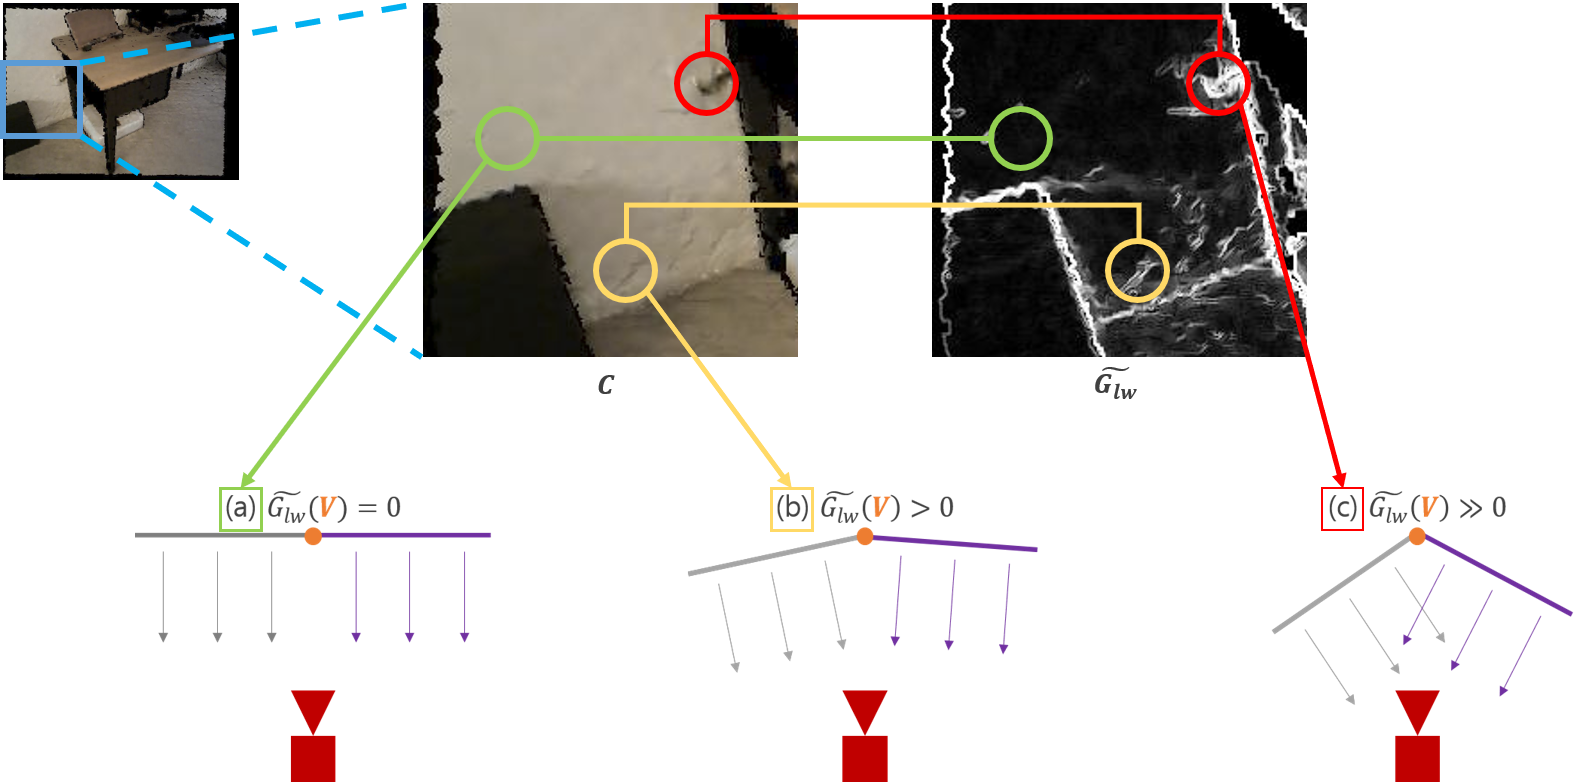
\includegraphics[width=\textwidth]{figures/3_method_relationship_gradient_lightweight_and_noise_full_tone_changed.png}
    \caption{Relationship between $G\textsubscript{lw}$ and actual noise of vertex $\textcolor{Orange}{V}$. We manually selected three pixels, where each have different magnitude of $G\textsubscript{lw}$. We also illustrated 1D example of the relationship. \textbf{\textcolor
    {Gray}{Gray}} and \textbf{\textcolor{Purple}{Purple}} lines and arrows indicate each face and its geometric normal. \textbf{\textcolor{LimeGreen}{(a)}} $\textcolor{Orange}{V}$ is considered as noise-free since $G\textsubscript{lw}$ is evaluated as zero, meaning adjacent faces have identical normal value. \textbf{\textcolor{Dandelion}{(b)}} $G\textsubscript{lw}$ is increased as two faces have inconsistent normal. \textbf{\textcolor{Red}{(c)}} as $G\textsubscript{lw}$ gets bigger, $\textcolor{Orange}{V}$ is considered as highly-noisy vertex. From these examples, we can say that $G\textsubscript{lw}$ precisely indicates where noisy pixels exist.}
    \label{fig:relationship_gradient_lightweight_and_noise}
\end{figure*}

\subsection{Optimization using Differentiable Rendering}
We define lightweight loss to minimize the difference between noise-free geometric information $\widetilde{G}_\mathcal{C}$ and noise-detected rendered image $\widetilde{G}_C$. We found that there is gradient value range inconsistency between $\widetilde{G}_\mathcal{C}$ and $\widetilde{G}_C$, as they are derived from different type of image i.e., color and geometry, respectively. We applied hyperbolic tangent kernel to each gradient image to ensure that both images have normalized value range, and we observed that this helped optimizer to find optimal without failure. Finally, we replace our target GT image from $\mathcal{C}$ to $\mathcal{C}\oplus\mathcal{D}$, as $\mathcal{M}$ follows holes where pixels in $\mathcal{D}$ have zero value. Our final geometric gradients are:
\begin{equation}
    G_\mathcal{C}=\tanh\left(\widetilde{G}_{\mathcal{C}\oplus\mathcal{D}}\right),
    G_{lw}=\tanh\left(\widetilde{G}_{lw}\right), 
\end{equation}
where $\tanh\left(x\right)=\frac{e^x-e^{-x}}{e^x+e^{-x}}$. Our optimizer minimizes lightweight loss representing geometric difference, while penalizing vertices not to evolve too far from its initial position:
\begin{gather}
    \mathcal{L}=w_{lw}\cdot L_{lw}+w_{pos}\cdot L_{pos}, \\
    L_{lw}=\left|\left|G_\mathcal{C}-G_C\right|\right|^2_2, \nonumber \\
    L_{pos}=\left|\left|V-\left(V_o\right)\right|\right|^2_2=\left|\left|V_d\right|\right|^2_2 \nonumber
\end{gather}
For all results, we used $w_{lw}=0.01$ and $w_{pos}=1.0$. Fig. 4 visualizes optimization procedure.
\begin{figure}
    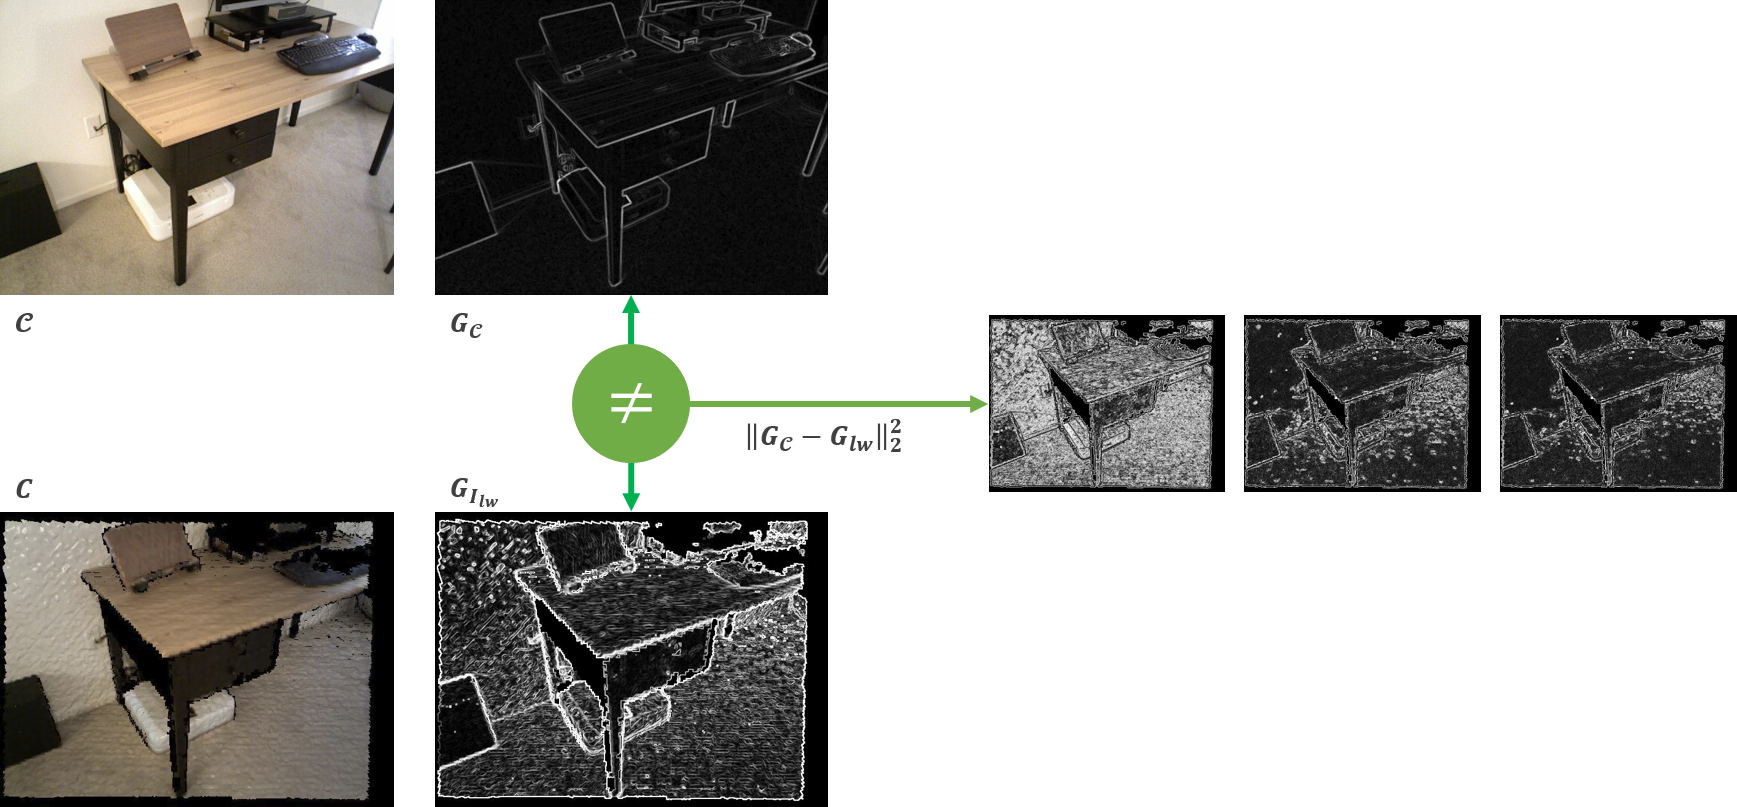
\includegraphics[width=\columnwidth]{figures/3_method_optimization.png}
    \caption{Optimization procedure of our differentiable rendering. From generated target noise-free geometric clue $G_\mathcal{C}$ and input noisy geometric clue $G_{lw}$, we minimize $L_2$ distance between two clues. Note that we additionally penalize aggressive vertex evolve, however it is skipped in the figure.}
    \label{fig:optimization}
\end{figure}